\documentclass[onlymath]{beamer}
% \documentclass[onlymath,handout]{beamer}

% Macros used by all lectures, but not necessarily by excercises

%%% General setup and dependencies:

% \usetheme[ddcfooter,nosectionnum]{tud}
\usetheme[nosectionnum,pagenum,noheader]{tud}
% \usetheme[nosectionnum,pagenum]{tud}

% Increase body font size to a sane level:
\let\origframetitle\frametitle
% \renewcommand{\frametitle}[1]{\origframetitle{#1}\normalsize}
\renewcommand{\frametitle}[1]{\origframetitle{#1}\fontsize{10pt}{13.2}\selectfont}
\setbeamerfont{itemize/enumerate subbody}{size=\small} % tud defaults to scriptsize!
\setbeamerfont{itemize/enumerate subsubbody}{size=\small}
% \setbeamerfont{normal text}{size=\small}
% \setbeamerfont{itemize body}{size=\small}

\renewcommand{\emph}[1]{\textbf{#1}}

\def\arraystretch{1.3}% Make tables even less cramped vertically

\usepackage[ngerman]{babel}
\usepackage[utf8]{inputenc}
\usepackage[T1]{fontenc}

%\usepackage{graphicx}
\usepackage[export]{adjustbox} % loads graphicx
\usepackage{import}
\usepackage{stmaryrd}
\usepackage[normalem]{ulem} % sout command
% \usepackage{times}
\usepackage{txfonts}

% \usepackage[perpage]{footmisc} % reset footnote counter on each page -- fails with beamer (footnotes gone)
\usepackage{perpage}  % reset footnote counter on each page
\MakePerPage{footnote}

\usepackage{tikz}
\usetikzlibrary{arrows,positioning}
% Inspired by http://www.texample.net/tikz/examples/hand-drawn-lines/
\usetikzlibrary{decorations.pathmorphing}
\pgfdeclaredecoration{penciline}{initial}{
    \state{initial}[width=+\pgfdecoratedinputsegmentremainingdistance,
    auto corner on length=1mm,]{
        \pgfpathcurveto%
        {% From
            \pgfqpoint{\pgfdecoratedinputsegmentremainingdistance}
                      {\pgfdecorationsegmentamplitude}
        }
        {%  Control 1
        \pgfmathrand
        \pgfpointadd{\pgfqpoint{\pgfdecoratedinputsegmentremainingdistance}{0pt}}
                    {\pgfqpoint{-\pgfdecorationsegmentaspect
                     \pgfdecoratedinputsegmentremainingdistance}%
                               {\pgfmathresult\pgfdecorationsegmentamplitude}
                    }
        }
        {%TO 
        \pgfpointadd{\pgfpointdecoratedinputsegmentlast}{\pgfpoint{1pt}{1pt}}
        }
    }
    \state{final}{}
}
\tikzset{handdrawn/.style={decorate,decoration=penciline}}
\tikzset{every shadow/.style={fill=none,shadow xshift=0pt,shadow yshift=0pt}}
% \tikzset{module/.append style={top color=\col,bottom color=\col}}

% Use to make Tikz attributes with Beamer overlays
% http://tex.stackexchange.com/a/6155
\tikzset{onslide/.code args={<#1>#2}{%
  \only<#1| handout:0>{\pgfkeysalso{#2}} 
}}
\tikzset{onslideprint/.code args={<#1>#2}{%
  \only<#1>{\pgfkeysalso{#2}} 
}}

%%% Title -- always set this first

\newcommand{\defineTitle}[3]{
	\newcommand{\lectureindex}{#1}
	\title{Formale Systeme}
	\subtitle{\href{\lectureurl}{#1. Vorlesung: #2}}
	\author{\href{http://korrekt.org/}{Markus Kr\"{o}tzsch}}
%	\author{\href{http://www.sebastian-rudolph.de}{Sebastian Rudolph} in Vertretung von \href{http://korrekt.org/}{Markus Kr\"{o}tzsch}}
	\date{#3}
	\datecity{TU Dresden}
% 	\institute{Computational Logic}
}

%%% Table of contents:

\RequirePackage{ifthen}

\newcommand{\highlight}[2]{%
	\ifthenelse{\equal{#1}{\lectureindex}}{\alert{#2}}{#2}%
}

\def\myspace{-0.7ex}
\newcommand{\printtoc}{
\begin{tabular}{r@{$\quad$}l}
\highlight{1}{1.} & \highlight{1}{Willkommen/Einleitung formale Sprachen}\\[\myspace]
\highlight{2}{2.} & \highlight{2}{Grammatiken und die Chomsky-Hierarchie}\\[\myspace]
\highlight{3}{3.} & \highlight{3}{Endliche Automaten}\\[\myspace]
\highlight{4}{4.} & \highlight{4}{Complexity of FO query answering}\\[\myspace]
\highlight{5}{5.} & \highlight{5}{Conjunctive queries}\\[\myspace]
\highlight{6}{6.} & \highlight{6}{Tree-like conjunctive queries}\\[\myspace]
\highlight{7}{7.} & \highlight{7}{Query optimisation}\\[\myspace]
\highlight{8}{8.} & \highlight{8}{Conjunctive Query Optimisation / First-Order~Expressiveness}\\[\myspace]
\highlight{9}{9.} & \highlight{9}{First-Order~Expressiveness / Introduction to Datalog}\\[\myspace]
\highlight{10}{10.} & \highlight{10}{Expressive Power and Complexity of Datalog}\\[\myspace]
\highlight{11}{11.} & \highlight{11}{Optimisation and Evaluation of Datalog}\\[\myspace]
\highlight{12}{12.} & \highlight{12}{Evaluation of Datalog (2)}\\[\myspace]
\highlight{13}{13.} & \highlight{13}{Graph Databases and Path Queries}\\[\myspace]
\highlight{14}{14.} & \highlight{14}{Outlook: database theory in practice}
\end{tabular}
}

\newcommand{\overviewslide}{%
\begin{frame}\frametitle{Overview}
\printtoc
\medskip

Siehe \href{\lectureurl}{course homepage [$\Rightarrow$ link]} for more information and materials
\end{frame}
}

%%% Colours:

\usepackage{xcolor,colortbl}
\definecolor{redhighlights}{HTML}{FFAA66}
\definecolor{lightblue}{HTML}{55AAFF}
\definecolor{lightred}{HTML}{FF5522}
\definecolor{lightpurple}{HTML}{DD77BB}
\definecolor{lightgreen}{HTML}{55FF55}
\definecolor{darkred}{HTML}{CC4411}
\definecolor{darkblue}{HTML}{176FC0}%{1133AA}
\definecolor{nightblue}{HTML}{2010A0}%{1133AA}
\definecolor{alert}{HTML}{176FC0}
\definecolor{darkgreen}{HTML}{36AB14}
\definecolor{strongyellow}{HTML}{FFE219}
\definecolor{devilscss}{HTML}{666666}

\newcommand{\redalert}[1]{\textcolor{darkred}{#1}}

%%% Style commands

\newcommand{\quoted}[1]{\texttt{"}{#1}\texttt{"}}
\newcommand{\squote}{\texttt{"}} % straight quote
\newcommand{\Sterm}[1]{\ensuremath{\mathtt{\textcolor{purple}{#1}}}}    % letters in alphabets
\newcommand{\Snterm}[1]{\textsf{\textcolor{darkblue}{#1}}} % nonterminal symbols
\newcommand{\Sntermsub}[2]{\Snterm{#1}_{\Snterm{#2}}} % nonterminal symbols
\newcommand{\Slang}[1]{\textbf{\textcolor{black}{#1}}}    % languages
\newcommand{\Slangsub}[2]{\Slang{#1}_{\Slang{#2}}}    % languages
% Code
\newcommand{\Scode}[1]{\textbf{#1}}    % reserved words in program listings, e.g., "if"
\newcommand{\Scodelit}[1]{\textcolor{purple}{#1}}    % literals in program listings, e.g., strings
\newcommand{\Scomment}[1]{\textcolor{gray}{#1}}    % comment in program listings

\newcommand{\epstrastar}{\mathrel{\mathord{\stackrel{\epsilon}{\to}}{}^*}} % transitive reflexive closure of epsilon transitions in an epslion-NFA

\newcommand{\narrowcentering}[1]{\mbox{}\hfill#1\hfill\mbox{}}

\newcommand{\defeq}{\mathrel{:=}}

\newcommand{\Smach}[1]{\ensuremath{\mathcal{#1}}}    % machines

%%% Slide layout commands:

\newcommand{\sectionSlide}[1]{
\frame{\begin{center}
\LARGE
#1
\end{center}}
}
\newcommand{\sectionSlideNoHandout}[1]{
\frame<handout:0>{\begin{center}
\LARGE
#1
\end{center}}
}

\newcommand{\mydualbox}[3]{%
 \begin{minipage}[t]{#1}
 \begin{beamerboxesrounded}[upper=block title,lower=block body,shadow=true]%
    {\centering\usebeamerfont*{block title}#2}%
    \raggedright%
    \usebeamerfont{block body}
%     \small
    #3%
  \end{beamerboxesrounded}
  \end{minipage}
}
% 
\newcommand{\myheaderbox}[2]{%
 \begin{minipage}[t]{#1}
 \begin{beamerboxesrounded}[upper=block title,lower=block title,shadow=true]%
    {\centering\usebeamerfont*{block title}\rule{0pt}{2.6ex} #2}%
  \end{beamerboxesrounded}
  \end{minipage}
}

\newcommand{\mycontentbox}[2]{%
 \begin{minipage}[t]{#1}%
 \begin{beamerboxesrounded}[upper=block body,lower=block body,shadow=true]%
    {\centering\usebeamerfont*{block body}\rule{0pt}{2.6ex}#2}%
  \end{beamerboxesrounded}
  \end{minipage}
}

\newcommand{\mylcontentbox}[2]{%
 \begin{minipage}[t]{#1}%
 \begin{beamerboxesrounded}[upper=block body,lower=block body,shadow=true]%
    {\flushleft\usebeamerfont*{block body}\rule{0pt}{2.6ex}#2}%
  \end{beamerboxesrounded}
  \end{minipage}
}

% label=180:{\rotatebox{90}{{\footnotesize\textcolor{darkgreen}{Beispiel}}}}
% \hspace{-8mm}\ghost{\raisebox{-7mm}{\rotatebox{90}{{\footnotesize\textcolor{darkgreen}{Beispiel}}}}}\hspace{8mm}
\newcommand{\examplebox}[1]{%
	\begin{tikzpicture}[decoration=penciline, decorate]
		\pgfmathsetseed{1235}
		\node (n1) [decorate,draw=darkgreen, fill=darkgreen!10,thick,align=left,text width=\linewidth, inner ysep=2mm, inner xsep=2mm] at (0,0) {#1};
% 		\node (n2) [align=left,text width=\linewidth,inner sep=0mm] at (n1.92) {{\footnotesize\raisebox{3mm}{\textcolor{darkgreen}{Beispiel}}}};
% 		\node (n2) [decorate,draw=darkgreen, fill=darkgreen!10,thick, align=left,text width=\linewidth,inner sep=2mm] at (n1.90) {{\footnotesize\raisebox{0mm}{\textcolor{darkgreen}{Beispiel}}}};
	\end{tikzpicture}%
}%

\newcommand{\codebox}[1]{%
	\begin{tikzpicture}[decoration=penciline, decorate]
		\pgfmathsetseed{1236}
		\node (n1) [decorate,draw=strongyellow, fill=strongyellow!10,thick,align=left,text width=\linewidth, inner ysep=2mm, inner xsep=2mm] at (0,0) {#1};
	\end{tikzpicture}%
}%

\newcommand{\defbox}[1]{%
	\begin{tikzpicture}[decoration=penciline, decorate]
		\pgfmathsetseed{1237}
		\node (n1) [decorate,draw=darkred, fill=darkred!10,thick,align=left,text width=\linewidth, inner ysep=2mm, inner xsep=2mm] at (0,0) {#1};
	\end{tikzpicture}%
}%

\newcommand{\theobox}[1]{%
	\begin{tikzpicture}[decoration=penciline, decorate]
		\pgfmathsetseed{1240}
		\node (n1) [decorate,draw=darkblue, fill=darkblue!10,thick,align=left,text width=\linewidth, inner ysep=2mm, inner xsep=2mm] at (0,0) {#1};
	\end{tikzpicture}%
}%

\newcommand{\anybox}[2]{%
	\begin{tikzpicture}[decoration=penciline, decorate]
		\pgfmathsetseed{1240}
		\node (n1) [decorate,draw=#1, fill=#1!10,thick,align=left,text width=\linewidth, inner ysep=2mm, inner xsep=2mm] at (0,0) {#2};
	\end{tikzpicture}%
}%


\newsavebox{\mybox}%
\newcommand{\doodlebox}[2]{%
\sbox{\mybox}{#2}%
	\begin{tikzpicture}[decoration=penciline, decorate]
		\pgfmathsetseed{1238}
		\node (n1) [decorate,draw=#1, fill=#1!10,thick,align=left,inner sep=1mm] at (0,0) {\usebox{\mybox}};
	\end{tikzpicture}%
}%

% Common notation

\usepackage{amsmath,amssymb,amsfonts}
\usepackage{xspace}

\newcommand{\lectureurl}{https://iccl.inf.tu-dresden.de/web/FS2016}

\DeclareMathAlphabet{\mathsc}{OT1}{cmr}{m}{sc} % Let's have \mathsc since the slide style has no working \textsc

% Dual of "phantom": make a text that is visible but intangible
\newcommand{\ghost}[1]{\raisebox{0pt}[0pt][0pt]{\makebox[0pt][l]{#1}}}

\newcommand{\tuple}[1]{\langle{#1}\rangle}

%%% Annotation %%%

\usepackage{color}
\newcommand{\todo}[1]{{\tiny\color{red}\textbf{TODO: #1}}}



%%% Old macros below; move when needed

\newcommand{\blank}{\text{\textvisiblespace}} % empty tape cell for TM

% table syntax
\newcommand{\dom}{\textbf{dom}}
\newcommand{\adom}{\textbf{adom}}
\newcommand{\dbconst}[1]{\texttt{"#1"}}
\newcommand{\pred}[1]{\textsf{#1}}
\newcommand{\foquery}[2]{#2[#1]}
\newcommand{\ground}[1]{\textsf{ground}(#1)}
% \newcommand{\foquery}[2]{\{#1\mid #2\}} %% Notation as used in Alice Book
% \newcommand{\foquery}[2]{\tuple{#1\mid #2}}

\newcommand{\quantor}{\mathord{\reflectbox{$\text{\sf{Q}}$}}} % the generic quantor

% logic syntax
\newcommand{\Inter}{\mathcal{I}} %used to denote an interpretation
\newcommand{\Jnter}{\mathcal{J}} %used to denote another interpretation
\newcommand{\Knter}{\mathcal{K}} %used to denote yet another interpretation
\newcommand{\Zuweisung}{\mathcal{Z}} %used to denote a variable assignment

% query languages
\newcommand{\qlang}[1]{{\sf #1}} % Font for query languages
\newcommand{\qmaps}[1]{\textbf{QM}({\sf #1})} % Set of query mappings for a query language

%%% Complexities %%%

\hyphenation{Exp-Time} % prevent "Ex-PTime" (see, e.g. Tobies'01, Glimm'07 ;-)
\hyphenation{NExp-Time} % better that than something else

% \newcommand{\complclass}[1]{{\sc #1}\xspace} % font for complexity classes
\newcommand{\complclass}[1]{\ensuremath{\mathsc{#1}}\xspace} % font for complexity classes

\newcommand{\ACzero}{\complclass{AC$_0$}}
\newcommand{\LogSpace}{\complclass{L}}
\newcommand{\NLogSpace}{\complclass{NL}}
\newcommand{\PTime}{\complclass{P}}
\newcommand{\NP}{\complclass{NP}}
\newcommand{\coNP}{\complclass{coNP}}
\newcommand{\PH}{\complclass{PH}}
\newcommand{\PSpace}{\complclass{PSpace}}
\newcommand{\NPSpace}{\complclass{NPSpace}}
\newcommand{\ExpTime}{\complclass{ExpTime}}
\newcommand{\NExpTime}{\complclass{NExpTime}}
\newcommand{\ExpSpace}{\complclass{ExpSpace}}
\newcommand{\TwoExpTime}{\complclass{2ExpTime}}
\newcommand{\NTwoExpTime}{\complclass{N2ExpTime}}
\newcommand{\ThreeExpTime}{\complclass{3ExpTime}}
\newcommand{\kExpTime}[1]{\complclass{#1ExpTime}}
\newcommand{\kExpSpace}[1]{\complclass{#1ExpSpace}}


\defineTitle{7}{Reguläre Ausdrücke}{3. November 2016}
\author{\href{http://korrekt.org/}{Markus Kr\"{o}tzsch}\\Daniel Borchmann}

\begin{document}

\maketitle

\begin{frame}\frametitle{}

% ~\hfill
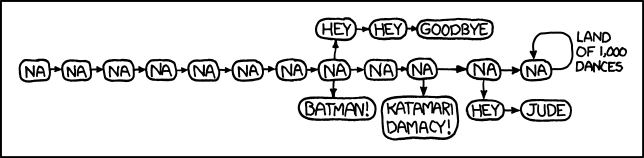
\includegraphics[width=10cm]{images/xkcd-na_make_it_better}
% \hfill~
% \rotatebox{90}

{\tiny Randall Munroe, \url{https://xkcd.com/851_make_it_better/}, CC-BY-NC 2.5}

\end{frame}

\sectionSlideNoHandout{Rückblick}


\begin{frame}\frametitle{Wiederholung: Reguläre Ausdrücke}

\begin{itemize}
\item Reguläre Ausdrücke als Syntax für Sprachen, die durch Operationen aus endlichen Sprachen gebildet werden
\item Grundformen: $\emptyset$, $\epsilon$, $\Sterm{a}$ für alle $\Sterm{a}\in\Sigma$
\item Operationen: Konkatenation, Alternative ($\mid$), Kleene-Stern (${}^*$)
\item Viele weitere Ausdrucksmittel in praktischen "`RegExps"'
\end{itemize}

\end{frame}

\begin{frame}\frametitle{Kleene's Theorem}

\theobox{Satz ("`Kleene's Theorem"'): Eine Sprache wird genau dann von einem regulären Ausdruck beschrieben, wenn sie von einem endlichen Automaten erkannt wird.}
\medskip

Letzte Vorlesung: "`regulärer Ausdruck $\leadsto$ endlicher Automat"'
\begin{itemize}
\item kompositionelle Methode
\item explizite Methode
\end{itemize}
\bigskip

Heute: "`endlicher Automat $\leadsto$ regulärer Ausdruck"'
\begin{itemize}
\item Ersetzungsmethode
\item Dynamische Programmierung
\end{itemize}


\hspace{8.1cm}\ghost{\raisebox{0.1cm}{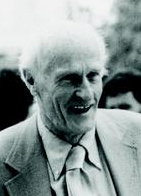
\includegraphics[height=3cm]{images/Kleene}~\rotatebox{90}{{\tiny Stephen Cole Kleene 1978 *}}}}

{\tiny *) Konrad Jacobs, Erlangen, \copyright{} Mathematisches Forschungsinstitut Oberwolfach, CC-BY-SA de 2.0}

% Hintergrund: Kleene (Aussprache "Klienie") war US Mathematiker -- im Gegensatz zum Linguisten Chomsky
% und dem Quereinsteiger Backus (die junge  Informatik im 20. Jhd wurde aus vielen Disziplinen gespeist).
% Kleene ist für eine Vielzahl an Beiträgen bekannt geworden. Ob "Kleene's Theorem" wirklich auf ihn zurueckgeht
% und wann bzw. wie er es bewiesen hat, ist mir nicht bekannt.

\end{frame}

\sectionSlide{Die Ersetzungsmethode}

\begin{frame}[fragile]\frametitle{Darstellungen von Typ-3-Sprachen}

\mbox{}\hspace{-0cm}%
\begin{tikzpicture}[
	decoration=penciline, decorate,
	node distance = 7mm and 9mm,
	mybox/.style args = {#1/#2}{
		draw=#1,% line color
		fill=#2,% fill color
% 		rounded corners,
		thick,
		text width=18mm, minimum height=12mm, inner sep=1mm,
		align=flush center
	},
	myboxlabel/.style args = {}{
		draw=devilscss,% line color
		fill=strongyellow!40,% fill color
% 		rounded corners,
		thick,
		text width=17mm, minimum height=10mm, inner sep=1.5mm,
		align=flush center
	},
	myarrow/.style args = {#1}{
		line width=0.8mm,
		draw=#1,%line color
		%-{Triangle[length=2.8mm,width=4mm,fill=#1]},
		->,
		shorten >=0.5mm, shorten <=0.1mm
	}
]
\pgfmathsetseed{7729}
% \draw[help lines] (0,0) grid (5,5);
\node (reg) [decorate,mybox=black/cyan!40] at (2,-0.6) {reguläre Grammatik};
\node (dfa) [decorate,mybox=black/cyan!40] at (0,-4) {DFA};
\node (nfa) [decorate,mybox=black/cyan!40] at (4,-4) {NFA};
\node (re) [decorate,mybox=black/cyan!40] at (6,-0.6) {regulärer Ausdruck};
\node (enfa) [decorate,mybox=black/cyan!40] at (8,-4) {$\epsilon$-NFA};
%
\path[myarrow=devilscss,bend left=20](dfa) edge (reg.180);
% \node (dfareglabel) [decorate,myboxlabel=,text width=19mm] at (-0.4,-0.7) {"`$q_1 \stackrel{\Sterm{a}}{\to} q_2$"' $\leadsto$ "`$q_1\to\Sterm{a}q_2$"'};
%
\path[myarrow=devilscss,-,bend left=20](reg.340) edge[->] (nfa.110);
\path[myarrow=devilscss,-,bend right=20](nfa.130) edge[->] (reg.320);
\node (regnfalabel) [decorate,myboxlabel=] at (1.6,-1.9) {\footnotesize"`$q_1\to\Sterm{a}q_2$"' $\Leftrightarrow$ "`$q_1 \stackrel{\Sterm{a}}{\to} q_2$"'};
%
\draw[myarrow=devilscss](dfa.10)--(nfa.170);
\node (dfanfalabel) [decorate,myboxlabel=,text width=16mm, minimum height=5mm,inner sep=1mm] at (1.95,-3.3) {\scalebox{0.8}{"`DFA${}\subseteq{}$NFA"'}};
%
\draw[myarrow=devilscss](nfa.190)--(dfa.350);
\node (nfadfalabel) [decorate,myboxlabel=,text width=13mm] at (2.1,-5.0) {\footnotesize Potenzm.\-konstr.};
%
\node (sd) [decorate,mybox=black/cyan!40,text width=14mm, minimum height=10mm] at (4,-6.5) {\footnotesize Syntax\-diagramm};
\draw[myarrow=devilscss,<->](sd)--(nfa);
\node (sdnfalabel) [decorate,myboxlabel=, minimum height=0mm,inner sep=1.0mm,text width=19mm] at (5.3,-5.4) {\footnotesize dualer Graph};
%%
\path[myarrow=devilscss,-,bend left=20,onslideprint={<2->{darkred}}](nfa.70) edge[->] (re.180);
%
\path[myarrow=devilscss,-,bend left=20](re.0) edge[->] (enfa);
%
\draw[myarrow=devilscss](enfa.190)--(nfa.350);
\draw[myarrow=devilscss](nfa.10)--(enfa.170);
\node (nfaenfalabel) [decorate,myboxlabel=,text width=16mm, minimum height=5mm,inner sep=1mm] at (5.95,-3.3) {\scalebox{0.75}{"`NFA${}\subseteq{}${}$\epsilon$-NFA"'}};
\node (enfanfalabel) [decorate,myboxlabel=,text width=13mm, minimum height=5mm] at (6.1,-4.6) {\footnotesize $\epsilon$-Elim.};
%
\node (nfarelabel) [decorate,myboxlabel=,align=flush left,text width=17mm,inner sep=1mm] at (8.6,-0.7) {\footnotesize 1) komposit.\\2) explizit};

%
\onslide<1>{\node (reenfalabel) [decorate,myboxlabel=,align=flush left,text width=18mm,inner sep=1mm] at (5.6,-2.0) {\footnotesize 1) Ersetzung\\2) Dyn. Prog.};}
\onslide<2->{\node (reenfalabel) [decorate,myboxlabel=,align=flush left,text width=18mm,inner sep=1mm] at (5.6,-2.0) {\footnotesize \redalert{1) Ersetzung}\\2) Dyn. Prog.};}
\end{tikzpicture}

\end{frame}

\begin{frame}\frametitle{NFA $\leadsto$ regulärer Ausdruck: Vorbereitung}

Wir vereinfachen den NFA zunächst wie folgt:

\codebox{
Gegeben: NFA  $\Smach{M}=\tuple{Q,\Sigma,\delta,Q_0,F}$
\begin{itemize}
\item Entferne alle Zustände, die von keinem Zustand in $Q_0$ erreichbar sind
\item Entferne alle Zustände, die von denen kein Zustand in $F$ erreichbar ist
\end{itemize}
Die Menge der von einem Zustand aus erreichbaren Zustände kann mit Graphalgorithmen berechnet werden, z.B. Breitensuche.
}

Offensichtlich verändert diese Vereinfachung die Sprache nicht
\pause

\doodlebox{darkgreen}{%
Beispiel: \hspace{6mm}
% \narrowcentering{%
\begin{tikzpicture}[baseline={(q1.base)}]
% \draw[help lines] (0,0) grid (7,2);
\node (q1) [circle,draw=black,thick] at (0,0) {$A$};
\node (q2) [circle,draw=black,thick] at (0,-1.5) {$B$};
\node (q12) [circle,draw=black,thick] at (2,0) {$C$};
\node (q22) [circle,draw=black,thick] at (2,-1.5) {$D$};
\node (q13) [circle,draw=black,thick,double] at (4,0) {$E$};
\node (q23) [circle,draw=black,thick] at (4,-1.5) {$F$};
\node (q14) [circle,draw=black,thick] at (6,0) {$G$};
\node (q24) [circle,draw=black,thick, double] at (6,-1.5) {$H$};
%
\path[->,line width=0.5mm](-0.7,0) edge (q1);
\path[->,line width=0.5mm](-0.7,-1.5) edge (q2);
\path[->,line width=0.5mm](q1) edge node[above] {\Sterm{a}} (q12);
\path[->,line width=0.5mm](q12) edge node[right] {\Sterm{b}} (q22);
\path[->,line width=0.5mm,bend left](q22) edge node[above] {\Sterm{b}} (q2);
\path[->,line width=0.5mm,bend left](q2) edge node[above] {\Sterm{a}} (q22);
\path[->,line width=0.5mm](q12) edge node[above] {\Sterm{a}} (q13);
\path[->,line width=0.5mm](q23) edge node[right] {\Sterm{a}} (q13);
\path[->,line width=0.5mm](q23) edge [loop left] node[left] {\Sterm{b}} (q23);
\path[->,line width=0.5mm](q24) edge node[above] {\Sterm{b}} (q23);
\path[->,line width=0.5mm](q24) edge node[right] {\Sterm{b}} (q14);
\path[->,line width=0.5mm](6.7,0) edge (q14);
%
\onslide<3->{
\node (cross1) at (0,-1.5) {\scalebox{4.0}{$\textcolor{darkred}{\boldsymbol{\times}}$}};
\node (cross2) at (2,-1.5) {\scalebox{4.0}{$\textcolor{darkred}{\boldsymbol{\times}}$}};
\node (cross3) at (4,-1.5) {\scalebox{4.0}{$\textcolor{darkred}{\boldsymbol{\times}}$}};
\node (cross4) at (6,-1.5) {\scalebox{4.0}{$\textcolor{darkred}{\boldsymbol{\times}}$}};
\node (cross5) at (6,0) {\scalebox{4.0}{$\textcolor{darkred}{\boldsymbol{\times}}$}};
}
\end{tikzpicture}\hspace{6mm}}

\end{frame}


\begin{frame}\frametitle{Die Ersetzungsmethode}

\emph{Gegeben:} NFA  $\Smach{M}=\tuple{Q,\Sigma,\delta,Q_0,F}$\\[1ex]
\emph{Gesucht:} regulärer Ausdruck $\alpha$ mit $\Slang{L}(\alpha)=\Slang{L}(\Smach{M})$\\[1ex]

\emph{Ansatz:}

\codebox{Für jeden Zustand $q\in Q$, berechne einen regulären Ausdruck $\alpha_q$ für die Sprache\\[-3ex]
\begin{align*}
\Slang{L}(\alpha_q) &=\{w\in\Sigma^*\mid \text{es gibt ein $q_f\in F$ mit }q\stackrel{w}{\to}q_f\} \\
	&= \{w\in\Sigma^*\mid \delta(q,w)\cap F\neq\emptyset\} \\
	&= \Slang{L}(\Smach{M}_q) \qquad \text{mit $\Smach{M}_q=\tuple{Q,\Sigma,\delta,\{q\},F}$}
\end{align*}
}

\emph{Dann gilt:}
\begin{align*}
\Slang{L}(\Smach{M}) &=\bigcup_{q\in Q_0} \Slang{L}(\alpha_q) \\
	&=  \Slang{L}(\alpha_{q_1}\mid\alpha_{q_2}\mid\ldots\mid \alpha_{q_n})\text{ mit }Q_0=\{q_1,q_2,\ldots,q_n\}
% 	&= \sum_{q\in Q_0} \alpha_q
\end{align*}

\end{frame}

\begin{frame}\frametitle{Notation}

Wir verwenden $\sum$ als verallgemeinerte Alternative:\medskip

\defbox{Für eine endliche Menge $A=\{\alpha_1,\ldots,\alpha_n\}$ von regulären Ausdrücken
schreiben wir $\sum_{\alpha\in A}\alpha$ als Abkürzung für $\alpha_1\mid\ldots\mid\alpha_n$.
}
\bigskip

Wir wenden diese Notation auch in anderen ähnlichen Fällen an, zum Beispiel für den vorigen Ausdruck:

\[\sum_{q\in Q_0} \alpha_q = \alpha_{q_1}\mid\alpha_{q_2}\mid\ldots\mid \alpha_{q_n}\]

\end{frame}

\begin{frame}\frametitle{Ersetzungsmethode -- Schwierigkeit}

Wie kann man die regulären Ausdrücke $\alpha_q$ finden?
\bigskip\pause

\doodlebox{darkgreen}{
\begin{minipage}{7cm}
\rule{0pt}{3ex}Beispiel: ohne Rekursion ist es einfach \ldots\\[1ex]

\begin{tikzpicture}[baseline={(q1.base)}]
% \draw[help lines] (0,0) grid (7,2);
\node (q1) [circle,draw=black,thick] at (0,0) {$A$};
\node (q12) [circle,draw=black,thick] at (2,0) {$C$};
\node (q13) [circle,draw=black,thick,double] at (4,0) {$E$};
%
\path[->,line width=0.5mm](-0.7,0) edge (q1);
\path[->,line width=0.5mm](q1) edge node[above] {\Sterm{a}} (q12);
\path[->,line width=0.5mm](q12) edge node[above] {\Sterm{a}} (q13);
%
\end{tikzpicture}\\
\end{minipage}
\begin{minipage}{2cm}
~\\$\alpha_A=\Sterm{aa}$,\\ $\alpha_C=\Sterm{a}$,\\ $\alpha_E=\Sterm{\epsilon}$
\end{minipage}
}\pause

\doodlebox{darkgreen}{
\begin{minipage}{7cm}
\rule{0pt}{3ex}Beispiel: mit Rekursion ist es weniger klar \ldots\\[1ex]

\narrowcentering{
\begin{tikzpicture}[baseline={(q1.base)}]
% \draw[help lines] (0,0) grid (7,2);
\node (q1) [circle,draw=black,thick] at (0,0) {$A$};
\node (q2) [circle,draw=black,thick] at (2,0) {$B$};
\node (q3) [circle,draw=black,thick,double] at (2,-1.7) {$C$};
%
\path[->,line width=0.5mm](-0.7,0) edge (q1);
\path[->,line width=0.5mm,bend right](q1) edge node[above] {\Sterm{a}} (q2);
\path[->,line width=0.5mm,bend right](q1) edge node[above] {\Sterm{b}} (q3);
\path[->,line width=0.5mm,bend left](q2) edge node[right] {\Sterm{a}} (q3);
\path[->,line width=0.5mm,bend left](q3) edge node[right] {\Sterm{b}} (q2);
\path[->,line width=0.5mm,bend right](q2) edge node[above] {\Sterm{a}} (q1);
\path[->,line width=0.5mm](q2) edge [loop right] node[right] {\Sterm{b}} (q2);
%
\end{tikzpicture}}\\
\end{minipage}
\begin{minipage}{2cm}
~\\$\alpha_A=?$\\
\end{minipage}
}

\end{frame}

\begin{frame}\frametitle{Ersetzungsmethode -- Rekursion}

\emph{Idee:} rekursiver Automat $\leadsto$ rekursive Definition von $\alpha_q$
\bigskip

Beispiel:

\narrowcentering{
\begin{tikzpicture}[baseline={(q1.base)}]
% \draw[help lines] (0,0) grid (7,2);
\node (q1) [circle,draw=black,thick] at (0,0) {$A$};
\node (q2) [circle,draw=black,thick] at (2,0) {$B$};
\node (q3) [circle,draw=black,thick,double,onslide={<10>{fill=strongyellow}}] at (2,-1.7) {$C$};
%
\path[->,line width=0.5mm](-0.7,0) edge (q1);
\path[->,line width=0.5mm,bend right,onslide={<2>{dashed,darkred}}](q1) edge node[above] {\Sterm{a}} (q2);
\path[->,line width=0.5mm,bend right,onslide={<3>{dashed,darkred}}](q1) edge node[above] {\Sterm{b}} (q3);
\path[->,line width=0.5mm,bend left,onslide={<6>{dashed,darkred}}](q2) edge node[right] {\Sterm{a}} (q3);
\path[->,line width=0.5mm,bend left,onslide={<9>{dashed,darkred}}](q3) edge node[right] {\Sterm{b}} (q2);
\path[->,line width=0.5mm,bend right,onslide={<5>{dashed,darkred}}](q2) edge node[above] {\Sterm{a}} (q1);
\path[->,line width=0.5mm,onslide={<7>{dashed,darkred}}](q2) edge [loop right] node[right] {\Sterm{b}} (q2);
%
\end{tikzpicture}}

\newcommand{\myequalityoverlay}{\only<-10|handout:0>{{}={}}\only<11->{{}\equiv{}}}
\hspace{4cm}% avoid jumping due to varying content length
$
\begin{array}{r@{}l}
\alpha_A & \myequalityoverlay\only<1|handout:0>{?}\onslide<2->{\Sterm{a}\alpha_B \mid{}}\only<2|handout:0>{\ldots}\onslide<3->{\Sterm{b}\alpha_C}\\
\alpha_B & \myequalityoverlay\only<1-4|handout:0>{?}\onslide<5->{\Sterm{a}\alpha_A \mid{}}\only<5|handout:0>{\ldots}\onslide<6->{\Sterm{a}\alpha_C \mid{}}\only<6|handout:0>{\ldots}\onslide<7->{\Sterm{b}\alpha_B}\\
\alpha_C & \myequalityoverlay\only<1-8|handout:0>{?}\onslide<9->{\Sterm{b}\alpha_B \mid{}}\only<9|handout:0>{\ldots}\onslide<10->{\epsilon}
\end{array}
$\bigskip

\onslide<11->{$\leadsto$ Ein \alert{Gleichungssystem} von regulären Ausdrücken!}

\end{frame}


\begin{frame}\frametitle{Ersetzungsmethode -- Gleichungen}

Allgemein kann man das Gleichungssystem wie folgt beschreiben:\medskip

\defbox{Für einen NFA $\Smach{M}=\tuple{Q,\Sigma,\delta,Q_0,F}$ betrachten wir
die folgenden Gleichungen für Ausdrücke $\alpha_q$ mit $q\in Q$.

\begin{itemize}
\item Für jeden Zustand $q\in Q\setminus F$:
\[ \alpha_q \equiv \sum_{\Sterm{a}\in\Sigma}\; \sum_{p\in\delta(q,\Sterm{a})} \Sterm{a}\alpha_p\]
\item Für jeden Zustand $q\in F$:
\[\alpha_q \equiv \epsilon \mid \sum_{\Sterm{a}\in\Sigma}\; \sum_{p\in\delta(q,\Sterm{a})} \Sterm{a}\alpha_p \]
\end{itemize}
}

Jetzt müssen wir diese Gleichungen lediglich lösen \ldots

\end{frame}


\begin{frame}\frametitle{Gleichungssysteme Lösen}

\examplebox{
\[ \alpha_A \equiv \Sterm{a}\alpha_B \mid \Sterm{b}\alpha_C \qquad
\alpha_B\equiv \Sterm{a}\alpha_A \mid\Sterm{a}\alpha_C \mid\Sterm{b}\alpha_B \qquad
\alpha_C \equiv \Sterm{b}\alpha_B \mid\epsilon\]
}

Wie können wir solche Gleichungssysteme lösen?\pause
\begin{itemize}
\item \emph{Methode 1:} Gleichungen ineinander Einsetzen und das Ergebnis vereinfachen\\[1ex]

\examplebox{
Beispiel: Setzen wir die Definition von $\alpha_C$ in die Gleichung für $\alpha_A$ ein, so erhalten wir
\[  \alpha_A \equiv \Sterm{a}\alpha_B \mid \Sterm{b}(\Sterm{b}\alpha_B \mid\epsilon) \equiv
\Sterm{a}\alpha_B \mid \Sterm{b}\Sterm{b}\alpha_B \mid \Sterm{b} \equiv (\Sterm{a} \mid \Sterm{b}\Sterm{b})\alpha_B \mid \Sterm{b}.\]}
Problem: rekursive Gleichungen lassen sich so nicht vereinfachen \ldots\pause
\item \emph{Methode 2:} Rekursive Gleichungen direkt Lösen\\
\theobox{\alert{Regel von Arden}: Aus $\alpha\equiv \beta\alpha\mid\gamma$ mit $\epsilon\notin\Slang{L}(\beta)$ folgt $\alpha\equiv\beta^*\gamma$.}
\end{itemize}

\end{frame}

\begin{frame}\frametitle{Beispiel: Gleichungssysteme Lösen}

\ghost{\hspace{5.5cm}\raisebox{-3.5cm}{\begin{minipage}{4cm}\onslide<5->{%
\theobox{\alert{Regel von Arden}:\\ Aus $\alpha\equiv \beta\alpha\mid\gamma$ mit $\epsilon\notin\Slang{L}(\beta)$ folgt $\alpha\equiv\beta^*\gamma$.}}
\end{minipage}}}

\begin{minipage}{5cm}
\begin{tikzpicture}[baseline={(q1.base)}]
% \draw[help lines] (0,0) grid (7,2);
\node (q1) [circle,draw=black,thick] at (0,0) {$1$};
\node (q2) [circle,draw=black,thick,double,onslide={<3>{fill=strongyellow}}] at (2,0) {$2$};
\node (q3) [circle,draw=black,thick,double,onslide={<4>{fill=strongyellow}}] at (0,-1.7) {$3$};
%
\path[->,line width=0.5mm](-0.7,0) edge (q1);
\path[->,line width=0.5mm,onslide={<2>{dashed,darkred}}](q1) edge node[above] {\Sterm{a}} (q2);
\path[->,line width=0.5mm,onslide={<2>{dashed,darkred}}](q1) edge node[right] {\Sterm{c}} (q3);
\path[->,line width=0.5mm,onslide={<3>{dashed,darkred}}](q2) edge [loop below] node[below] {\Sterm{b}} (q2);
%
\end{tikzpicture}
\end{minipage}
\begin{minipage}{3cm}\pause
\begin{tabular}{rl}
(1)& $\alpha_1 \equiv \Sterm{a}\alpha_2 \mid \Sterm{c}\alpha_3 $\\\pause
(2)& $\alpha_2 \equiv \Sterm{b}\alpha_2 \mid\epsilon $\\\pause
(3)& $\alpha_3 \equiv \epsilon$
\end{tabular}
\end{minipage}\medskip\pause\pause


\begin{tabular}{rll}
(4) & $\alpha_2 \equiv \Sterm{b}^*\epsilon \equiv \Sterm{b}^*$ & Arden (2)\\\pause
%
(5) & $\alpha_1 \equiv \Sterm{a}\Sterm{b}^*\mid \Sterm{c}\alpha_3$ & (4) in (1)\\\pause
%
(6) & $\alpha_1 \equiv \Sterm{a}\Sterm{b}^*\mid \Sterm{c}$ & (3) in (5)\\\pause
\end{tabular}

$\leadsto$ regulärer Ausdruck für NFA ist $\sum_{q\in Q_0}\alpha_q = \alpha_1$, also $\Sterm{a}\Sterm{b}^*\mid \Sterm{c}$

\end{frame}

%
% \begin{frame}\frametitle{Beispiel: Gleichungssysteme Lösen}
%
% \begin{minipage}{5cm}
% \begin{tikzpicture}[baseline={(q1.base)}]
% % \draw[help lines] (0,0) grid (7,2);
% \node (q1) [circle,draw=black,thick] at (0,0) {$A$};
% \node (q2) [circle,draw=black,thick] at (2,0) {$B$};
% \node (q3) [circle,draw=black,thick,double] at (2,-1.7) {$C$};
% %
% \path[->,line width=0.5mm](-0.7,0) edge (q1);
% \path[->,line width=0.5mm,bend right](q1) edge node[above] {\Sterm{a}} (q2);
% \path[->,line width=0.5mm,bend right](q1) edge node[above] {\Sterm{b}} (q3);
% \path[->,line width=0.5mm,bend left](q2) edge node[right] {\Sterm{a}} (q3);
% \path[->,line width=0.5mm,bend left](q3) edge node[right] {\Sterm{b}} (q2);
% \path[->,line width=0.5mm,bend right](q2) edge node[above] {\Sterm{a}} (q1);
% \path[->,line width=0.5mm](q2) edge [loop right] node[right] {\Sterm{b}} (q2);
% %
% \end{tikzpicture}
% \end{minipage}
% \begin{minipage}{3cm}
% \begin{align*}
% (1)&& \alpha_A &\equiv \Sterm{a}\alpha_B \mid \Sterm{b}\alpha_C \\
% (2)&& \alpha_B &\equiv \Sterm{a}\alpha_A \mid\Sterm{a}\alpha_C \mid\Sterm{b}\alpha_B \\
% (3)&& \alpha_C &\equiv \Sterm{b}\alpha_B \mid\epsilon
% \end{align*}
% \end{minipage}\pause
%
% \begin{tabular}{rll}
% $(4)$ & $\alpha_A \equiv (\Sterm{a} \mid \Sterm{b}\Sterm{b})\alpha_B \mid \Sterm{b}$ & $(3)$ in $(1)$\\\pause
% %
% $(5)$ & $\alpha_B \equiv \Sterm{a}\alpha_A \mid\Sterm{a}(\Sterm{b}\alpha_B \mid\epsilon) \mid\Sterm{b}\alpha_B \equiv
% \Sterm{a}\alpha_A \mid (\Sterm{ab}\mid\Sterm{b})\alpha_B  \mid \Sterm{a}$ & $(3)$ in $(2)$\\\pause
% %
% $(6)$ &
% $\alpha_B \equiv \Sterm{a}((\Sterm{a} \mid \Sterm{b}\Sterm{b})\alpha_B \mid \Sterm{b}) \mid (\Sterm{ab}\mid\Sterm{b})\alpha_B  \mid \Sterm{a}$ & $(4)$ in $(5)$\\
% & $\phantom{\alpha_B}\equiv (\Sterm{aa} \mid \Sterm{abb}\mid\Sterm{ab}\mid\Sterm{b})\alpha_B \mid \Sterm{ab}  \mid \Sterm{a}$
% \\\pause
% %
% $(7)$ &
% $\alpha_B\equiv (\Sterm{aa} \mid \Sterm{abb}\mid\Sterm{ab}\mid\Sterm{b})^* (\Sterm{ab}  \mid \Sterm{a})$
% & Arden $(6)$\\\pause
% %
% $(8)$ &
% $\alpha_A \equiv (\Sterm{a} \mid \Sterm{b}\Sterm{b})(\Sterm{aa} \mid \Sterm{abb}\mid\Sterm{ab}\mid\Sterm{b})^* (\Sterm{ab}  \mid \Sterm{a}) \mid \Sterm{b}$
% & $(6)$ in $(4)$\\\pause
% %
% $(9)$ &
% $\alpha_C \equiv \Sterm{b}(\Sterm{aa} \mid \Sterm{abb}\mid\Sterm{ab}\mid\Sterm{b})^* (\Sterm{ab}  \mid \Sterm{a}) \mid\epsilon$
% & $(6)$ in $(3)$
% \end{tabular}
%
% \end{frame}

\begin{frame}\frametitle{Korrektheit der Ersetzungsregel (1)}

\theobox{\alert{Regel von Arden${}^*$}: Aus $\alpha\equiv \beta\alpha\mid\gamma$ mit $\epsilon\notin\Slang{L}(\beta)$ folgt $\alpha\equiv\beta^*\gamma$.}

\emph{Beweis:} Wir behaupten: Wenn $\Slang{L}(\alpha)= \Slang{L}(\beta)\circ \Slang{L}(\alpha)\cup\Slang{L}(\gamma)$ mit $\epsilon\notin\Slang{L}(\beta)$ dann gilt $\Slang{L}(\alpha)=\Slang{L}(\beta)^*\circ\Slang{L}(\gamma)$.
\bigskip

Wir zeigen: dies gilt nicht nur für $\Slang{L}(\alpha)$, $\Slang{L}(\beta)$ und $\Slang{L}(\gamma)$, sondern für beliebige Sprachen $\Slang{L}$, $\Slang{K}$ und $\Slang{H}$:
\bigskip

\narrowcentering{
Wenn $\Slang{L}= \Slang{K}\Slang{L}\cup\Slang{H}$ und $\epsilon\notin\Slang{K}$ dann $\Slang{L}=\Slang{K}^*\Slang{H}$}
\bigskip

Wir zeigen die beiden Richtungen der geforderten Gleichheit einzeln.
\bigskip

{\tiny \alert{${}^*$ nach Dean N. Arden der das Resultat 1961 publizierte; auch bekannt als "`Lemma von Arden"'}}

% Über DN Arden gibt es sonst wenig verbriefte Informationen. DBLP listet nur diese einzige Publikation.
% Wikipedia hat keine Artikel zu seiner Person. Auch ein Bild konnte ich nicht finden.
% Das Resultat selbst ist von historischer Bedeutung, da es eine der ersten Ergebnisse zu Fixpunkt-Berechnungen in
% der Informatik darstellt.

\end{frame}

\begin{frame}[t]\frametitle{Korrektheit der Ersetzungsregel (2)}

\emph{Annahme:} $\Slang{L}= \Slang{K}\Slang{L}\cup\Slang{H}$ und $\epsilon\notin\Slang{K}$\\[1ex]

\emph{Teilbehauptung 1:} $\Slang{K}^*\Slang{H}\subseteq\Slang{L}$\pause\\[1ex]

\begin{itemize}
\item Sei $w\in \Slang{K}^*\Slang{H}$ beliebig\pause
\item Dann hat $w$ die Form $u_1\cdots u_n v$ mit $n\geq 0$, $u_1,\ldots,u_n\in\Slang{K}$ und $v\in\Slang{H}$\pause
\item Wegen $\Slang{L}= \Slang{K}\Slang{L}\cup\Slang{H}$ gilt $\Slang{K}\Slang{L}\subseteq\Slang{L}$ und $\Slang{H}\subseteq\Slang{L}$\pause
\item Wegen $v\in\Slang{H}$ und $\Slang{H}\subseteq\Slang{L}$ gilt $v\in\Slang{L}$\pause
\item Wegen $v\in\Slang{L}$, $u_n\in\Slang{K}$ und $\Slang{K}\Slang{L}\subseteq\Slang{L}$ gilt $u_n v\in\Slang{L}$\pause
\item Wegen $u_n v\in\Slang{L}$, $u_{n-1}\in\Slang{K}$ und $\Slang{K}\Slang{L}\subseteq\Slang{L}$ gilt $u_{n-1} u_n v\in\Slang{L}$\pause\\
\ldots
\item Wegen $u_2\cdots u_n v\in\Slang{L}$, $u_1\in\Slang{K}$ und $\Slang{K}\Slang{L}\subseteq\Slang{L}$ gilt $\underbrace{u_1\cdots u_n v}_w\in\Slang{L}$
\end{itemize}

\end{frame}

\begin{frame}[t]\frametitle{Korrektheit der Ersetzungsregel (3)}

\emph{Annahme:} $\Slang{L}= \Slang{K}\Slang{L}\cup\Slang{H}$ und $\epsilon\notin\Slang{K}$\\[1ex]

\emph{Teilbehauptung 2:} $\Slang{L}\subseteq\Slang{K}^*\Slang{H}$\pause\\[1ex]

Sei $w\in \Slang{L}$ beliebig. Wir beweisen $w\in\Slang{K}^*\Slang{H}$ durch Induktion über $|w|$.
\medskip

\alert{Induktionsanfang:} sei $n=0$\pause
\begin{itemize}
\item Dann ist $w=\epsilon$\pause
\item Weil $\epsilon\notin\Slang{K}$ gilt $\epsilon\notin\Slang{K}\Slang{L}$\pause
\item Da $w=\epsilon\in\Slang{L}$ und $\Slang{L}= \Slang{K}\Slang{L}\cup\Slang{H}$ gilt also $\epsilon\in\Slang{H}$\pause
\item Also gilt $w\in\Slang{K}^*\Slang{H}$.
\end{itemize}

\end{frame}

\begin{frame}[t]\frametitle{Korrektheit der Ersetzungsregel (4)}

\emph{Annahme:} $\Slang{L}= \Slang{K}\Slang{L}\cup\Slang{H}$ und $\epsilon\notin\Slang{K}$\\[1ex]

\emph{Teilbehauptung 2:} $\Slang{L}\subseteq\Slang{K}^*\Slang{H}$\\[1ex]

% Sei $w\in \Slang{L}$ beliebig. Wir beweisen $w\in\Slang{K}^*\Slang{H}$ durch Induktion über $|w|$.
\medskip

\alert{Induktionshypothese:} Die Aussage gilt für alle Wörter $v$ mit $|v|<n$, d.h., für jedes solches $v\in\Slang{L}$ gilt auch $v\in\Slang{K}^*\Slang{H}$ \pause
\medskip

\alert{Induktionsschritt:} sei $|w|=n$\pause
\begin{itemize}
\item Wegen $\Slang{L}= \Slang{K}\Slang{L}\cup\Slang{H}$ gilt (1) $w\in\Slang{H}$ oder (2) $w\in \Slang{K}\Slang{L}$\pause
\item Fall 1 $w\in\Slang{H}$: dann ist $w=\epsilon w \in \Slang{K}^*\Slang{H}$\pause
\item Fall 2 $w\in \Slang{K}\Slang{L}$\pause:
	\begin{itemize}
	\item Dann gibt es $u\in\Slang{K}$ und $v\in\Slang{L}$ mit $w=uv$\pause
	\item Wegen $\epsilon\notin\Slang{K}$ ist $u\neq\epsilon$ und also $|v|<|w|=n$\pause
	\item Laut IH gilt also $v\in\Slang{K}^*\Slang{H}$\pause
	\item Wegen $u\in\Slang{K}$ gilt also auch $uv=w\in\Slang{K}^*\Slang{H}$
	\end{itemize}
\end{itemize}

Damit ist der Beweis abgeschlossen.\qed

\end{frame}

\begin{frame}\frametitle{Zusammenfassung Ersetzungsmethode}

Die Umwandlung NFA $\leadsto$ regulärer Ausdruck ist also wie folgt:

\begin{enumerate}[(1)]
\item \alert{Vereinfache den Automaten} (entferne offensichtlich unnötige Zustände)
\item \alert{Bestimme das Gleichungssystem} (eine Gleichung pro Zustand)
\item \alert{Löse das Gleichungssystem} (durch Einsetzen und Ardens Regel)
\item \alert{Gib den Ausdruck für die Sprache des NFA an} (Alternative der Ausdrücke für alle Anfangszustände)
\end{enumerate}

\end{frame}


\sectionSlide{Ermittlung regulärer Ausdrücke durch dynamische Programmierung}

\begin{frame}[fragile]\frametitle{Darstellungen von Typ-3-Sprachen}

\mbox{}\hspace{-0cm}%
\begin{tikzpicture}[
	decoration=penciline, decorate,
	node distance = 7mm and 9mm,
	mybox/.style args = {#1/#2}{
		draw=#1,% line color
		fill=#2,% fill color
% 		rounded corners,
		thick,
		text width=18mm, minimum height=12mm, inner sep=1mm,
		align=flush center
	},
	myboxlabel/.style args = {}{
		draw=devilscss,% line color
		fill=strongyellow!40,% fill color
% 		rounded corners,
		thick,
		text width=17mm, minimum height=10mm, inner sep=1.5mm,
		align=flush center
	},
	myarrow/.style args = {#1}{
		line width=0.8mm,
		draw=#1,%line color
		%-{Triangle[length=2.8mm,width=4mm,fill=#1]},
		->,
		shorten >=0.5mm, shorten <=0.1mm
	}
]
\pgfmathsetseed{7729}
% \draw[help lines] (0,0) grid (5,5);
\node (reg) [decorate,mybox=black/cyan!40] at (2,-0.6) {reguläre Grammatik};
\node (dfa) [decorate,mybox=black/cyan!40] at (0,-4) {DFA};
\node (nfa) [decorate,mybox=black/cyan!40] at (4,-4) {NFA};
\node (re) [decorate,mybox=black/cyan!40] at (6,-0.6) {regulärer Ausdruck};
\node (enfa) [decorate,mybox=black/cyan!40] at (8,-4) {$\epsilon$-NFA};
%
\path[myarrow=devilscss,bend left=20](dfa) edge (reg.180);
% \node (dfareglabel) [decorate,myboxlabel=,text width=19mm] at (-0.4,-0.7) {"`$q_1 \stackrel{\Sterm{a}}{\to} q_2$"' $\leadsto$ "`$q_1\to\Sterm{a}q_2$"'};
%
\path[myarrow=devilscss,-,bend left=20](reg.340) edge[->] (nfa.110);
\path[myarrow=devilscss,-,bend right=20](nfa.130) edge[->] (reg.320);
\node (regnfalabel) [decorate,myboxlabel=] at (1.6,-1.9) {\footnotesize"`$q_1\to\Sterm{a}q_2$"' $\Leftrightarrow$ "`$q_1 \stackrel{\Sterm{a}}{\to} q_2$"'};
%
\draw[myarrow=devilscss](dfa.10)--(nfa.170);
\node (dfanfalabel) [decorate,myboxlabel=,text width=16mm, minimum height=5mm,inner sep=1mm] at (1.95,-3.3) {\scalebox{0.8}{"`DFA${}\subseteq{}$NFA"'}};
%
\draw[myarrow=devilscss](nfa.190)--(dfa.350);
\node (nfadfalabel) [decorate,myboxlabel=,text width=13mm] at (2.1,-5.0) {\footnotesize Potenzm.\-konstr.};
%
\node (sd) [decorate,mybox=black/cyan!40,text width=14mm, minimum height=10mm] at (4,-6.5) {\footnotesize Syntax\-diagramm};
\draw[myarrow=devilscss,<->](sd)--(nfa);
\node (sdnfalabel) [decorate,myboxlabel=, minimum height=0mm,inner sep=1.0mm,text width=19mm] at (5.3,-5.4) {\footnotesize dualer Graph};
%%
\path[myarrow=devilscss,-,bend left=20,darkred](nfa.70) edge[->] (re.180);
%
\path[myarrow=devilscss,-,bend left=20](re.0) edge[->] (enfa);
%
\draw[myarrow=devilscss](enfa.190)--(nfa.350);
\draw[myarrow=devilscss](nfa.10)--(enfa.170);
\node (nfaenfalabel) [decorate,myboxlabel=,text width=16mm, minimum height=5mm,inner sep=1mm] at (5.95,-3.3) {\scalebox{0.75}{"`NFA${}\subseteq{}${}$\epsilon$-NFA"'}};
\node (enfanfalabel) [decorate,myboxlabel=,text width=13mm, minimum height=5mm] at (6.1,-4.6) {\footnotesize $\epsilon$-Elim.};
%
\node (nfarelabel) [decorate,myboxlabel=,align=flush left,text width=17mm,inner sep=1mm] at (8.6,-0.7) {\footnotesize 1) komposit.\\2) explizit};

%
{\node (reenfalabel) [decorate,myboxlabel=,align=flush left,text width=18mm,inner sep=1mm] at (5.6,-2.0) {\footnotesize 1) Ersetzung\\\redalert{2) Dyn. Prog.}};}
\end{tikzpicture}

\end{frame}

\begin{frame}\frametitle{Idee}

\emph{Gegeben:} NFA  $\Smach{M}=\tuple{Q,\Sigma,\delta,Q_0,F}$\\[1ex]
\emph{Gesucht:} regulärer Ausdruck $\alpha$ mit $\Slang{L}(\alpha)=\Slang{L}(\Smach{M})$\\[1ex]

\emph{Ansatz:}

\codebox{Für jedes Paar von Zuständen $q,p\in Q$, berechne einen regulären Ausdruck $\alpha_{q,p}$ für die Sprache\\[-3ex]
\begin{align*}
\Slang{L}(\alpha_{q,p}) &=\{w\in\Sigma^*\mid q\stackrel{w}{\to}p\} \\
	&= \{w\in\Sigma^*\mid p\in\delta(q,w)\} \\
	&= \Slang{L}(\Smach{M}_{q,p}) \qquad \text{mit $\Smach{M}_{q,p}=\tuple{Q,\Sigma,\delta,\{q\},\{p\}}$}
\end{align*}
}

\emph{Dann gilt:}
\begin{align*}
\Slang{L}(\Smach{M}) &=\bigcup_{q\in Q_0} \bigcup_{p\in F} \Slang{L}(\alpha_{q,p})
	=  \Slang{L}\left(\sum_{q\in Q_0} \sum_{p\in F} \alpha_{q,p}\right)
\end{align*}

\end{frame}

\newcommand{\Lijk}[3]{\ensuremath{\Slang{L}^{#3}[#1,#2]}}
\newcommand{\alphaijk}[3]{\ensuremath{\alpha^{#3}[#1,#2]}}

\begin{frame}\frametitle{Dynamische Ermittlung von $\alpha_{q,p}$}

\emph{Gegeben:} NFA  $\Smach{M}=\tuple{Q,\Sigma,\delta,Q_0,F}$\\[1ex]
\emph{Annahme:} Zustände sind nummeriert: $Q=\{q_1,\ldots,q_n\}$ (o.b.d.A.)\\[1ex]

\defbox{Gegeben $\Smach{M}$, Zahlen $i,j\in\{1,\ldots,n\}$ und eine Zahl $k\in\{0,1,\ldots,n\}$ definieren wir die Sprache $\Lijk{i}{j}{k}$ als
die Menge aller Wörter $w=\Sterm{a_1}\cdots\Sterm{a_\ell}$ für die gilt:
\begin{itemize}
\item es gibt einen Lauf $q_i\stackrel{\Sterm{a_1}}{\to}p_1\stackrel{\Sterm{a_2}}{\to}\ldots\stackrel{\Sterm{a_{\ell-1}}}{\to}p_{\ell-1}\stackrel{\Sterm{a_\ell}}{\to}q_j$, wobei
\item für jeden Zwischenzustand $p_i$ mit $i\in\{1,\ldots,\ell-1\}$ gilt $p_i\in\{q_1,\ldots,q_k\}$
\end{itemize}
}

\emph{Gesucht:} Reguläre Ausdrücke $\alphaijk{i}{j}{k}$ mit $\Slang{L}(\alphaijk{i}{j}{k})=\Lijk{i}{j}{k}$.
\medskip

\alert{Wir wollen dynamische Programmierung anwenden, um $\alphaijk{i}{j}{k}$ für immer größere Werte $k$ zu berechnen.}

\end{frame}

\begin{frame}[t]\frametitle{Der Fall $k=n$}

\defbox{Gegeben $\Smach{M}$, Zahlen $i,j\in\{1,\ldots,n\}$ und eine Zahl $k\in\{0,1,\ldots,n\}$ definieren wir die Sprache $\Lijk{i}{j}{k}$ als
die Menge aller Wörter $w=\Sterm{a_1}\cdots\Sterm{a_\ell}$ für die gilt:

\begin{itemize}
\item es gibt einen Lauf $q_i\stackrel{\Sterm{a_1}}{\to}p_1\stackrel{\Sterm{a_2}}{\to}\ldots\stackrel{\Sterm{a_{\ell-1}}}{\to}p_{\ell-1}\stackrel{\Sterm{a_\ell}}{\to}q_j$, wobei
\item für jeden Zwischenzustand $p_i$ mit $i\in\{1,\ldots,\ell-1\}$ gilt $p_i\in\{q_1,\ldots,q_k\}$
\end{itemize}
}
% \medskip

Für $k=n$ ist die zweite Bedingung immer erfüllt, da $\{q_1,\ldots,q_n\}=Q$\\[1ex]
%
$\leadsto$ $\Lijk{i}{j}{n}$ ist die Menge aller Wörter "`zwischen"' $q_i$ und $q_j$\\[1ex]
%
$\leadsto$ $\alphaijk{i}{j}{n} = \alpha_{q_i,q_j}$ sind die regulären Ausdrücke, aus denen wir letztlich die Lösung ermitteln wollen
\end{frame}

\begin{frame}[t]\frametitle{Der Fall $k=0$}

\defbox{Gegeben $\Smach{M}$, Zahlen $i,j\in\{1,\ldots,n\}$ und eine Zahl $k\in\{0,1,\ldots,n\}$ definieren wir die Sprache $\Lijk{i}{j}{k}$ als
die Menge aller Wörter $w=\Sterm{a_1}\cdots\Sterm{a_\ell}$ für die gilt:

\begin{itemize}
\item es gibt einen Lauf $q_i\stackrel{\Sterm{a_1}}{\to}p_1\stackrel{\Sterm{a_2}}{\to}\ldots\stackrel{\Sterm{a_{\ell-1}}}{\to}p_{\ell-1}\stackrel{\Sterm{a_\ell}}{\to}q_j$, wobei
\item für jeden Zwischenzustand $p_i$ mit $i\in\{1,\ldots,\ell-1\}$ gilt $p_i\in\{q_1,\ldots,q_k\}$
\end{itemize}
}
% \medskip

Für $k=0$ kann die zweite Bedingung für keinen Zustand $p_i$ erfüllt werden\\[1ex]
%
$\leadsto$ $\Lijk{i}{j}{0}$ beruht nur auf Läufen ohne Zwischenzustände
%
\begin{itemize}
\item Falls $i\neq j$, dann kommen nur Läufe $q_i\stackrel{\Sterm{a}}{\to}q_j$ in Frage
\item Falls $i=j$, dann kommen Läufe $q_i\stackrel{\Sterm{a}}{\to}q_i$ ($w=\Sterm{a}$) oder $q_i$ ($w=\epsilon$) in Frage
\end{itemize}
%
$\leadsto$ reguläre Ausdrücke $\alphaijk{i}{j}{0}$ können direkt aus $\Smach{M}$ abgelesen werden

\end{frame}

\begin{frame}\frametitle{Die regulären Ausdrücke $\alphaijk{i}{j}{0}$}

Für $k=0$ können wir $\alphaijk{i}{j}{0}$ direkt aus $\Smach{M}$ ablesen:
\bigskip

\codebox{
Sei $\{\Sterm{a_1},\ldots,\Sterm{a_m}\}=\{\Sterm{a}\in\Sigma\mid q_i\stackrel{\Sterm{a}}{\to}q_j\}$ die Menge der Beschriftungen von direkten Übergängen von $q_i$ zu $q_j$.

\begin{itemize}
\item Falls $i\neq j$, dann ist
\[\alphaijk{i}{j}{0} = \Sterm{a_1}\mid\ldots\mid\Sterm{a_m}\]
\item Falls $i=j$, dann ist
\[\alphaijk{i}{j}{0} = \Sterm{a_1}\mid\ldots\mid\Sterm{a_m}\mid\epsilon\]
\end{itemize}
}

\end{frame}

\begin{frame}\frametitle{Die regulären Ausdrücke $\alphaijk{i}{j}{k+1}$}

Zur Bestimmung von $\alphaijk{i}{j}{k+1}$ verwenden wir Ausdrücke $\alphaijk{i'}{j'}{k}$
\bigskip

\defbox{\vspace{-0.5ex}\begin{itemize}
\item es gibt einen Lauf $q_i\stackrel{\Sterm{a_1}}{\to}p_1\stackrel{\Sterm{a_2}}{\to}\ldots\stackrel{\Sterm{a_{\ell-1}}}{\to}p_{\ell-1}\stackrel{\Sterm{a_\ell}}{\to}q_j$, wobei
\item für jedes $p_i$ mit $i\in\{1,\ldots,\ell-1\}$ gilt $p_i\in\{q_1,\ldots,q_k\}$
\end{itemize}
}

$\leadsto$ zwei Möglichkeiten für Läufe bei $k+1$:
\begin{enumerate}[(1)]
\item kein $p_i$ ist $q_{k+1}$, d.h. $p_i\in\{q_1,\ldots,q_k\}$
\item einige $p_i$ sind $q_{k+1}$; dann hat der Lauf die Form:
\end{enumerate}
\[ %q_i \{q_1,\ldots,q_k \}^* q_{k+1} \big( \{q_1,\ldots,q_k \}^* q_{k+1}\big)^* \{q_1,\ldots,q_k \}^*q_j
\begin{array}{@{}r@{}r@{}c@{}r@{}c@{}r@{}c@{}l@{}}
&
q_i & \textcolor{black}{\{q_1,\ldots,q_k \}^*} & q_{k+1}\big( &  \textcolor{black}{\{q_1,\ldots,q_k \}^*}q_{k+1}  & \big)^* & \textcolor{black}{\{q_1,\ldots,q_k \}^*} & q_j \\
{\footnotesize\text{Teilläufe:}} &
    & {\footnotesize\text{\textcolor{darkred}{$q_i\to q_{k+1}$}}} &  ( & {\footnotesize\text{\textcolor{darkblue}{$q_{k+1}\to q_{k+1}$}}} & )^* & {\footnotesize\text{\textcolor{darkgreen}{$q_{k+1}\to q_j$}}} & \\
\end{array}
\]
% \[ q_i\stackrel{\Sterm{a_1}}{\to}p_1\stackrel{\Sterm{a_2}}{\to}\ldots\stackrel{\Sterm{a_{\ell-1}}}{\to}p_{\ell-1}\stackrel{\Sterm{a_\ell}}{\to}q_j \]
% \medskip

Daher gilt:
\codebox{\vspace{-1.5ex}
\[\alphaijk{i}{j}{k+1} = \underbrace{\alphaijk{i}{j}{k}}_{\text{Fall (1)}} \mid \underbrace{\big( \textcolor{darkred}{\alphaijk{i}{k+1}{k}} (\textcolor{darkblue}{\alphaijk{k+1}{k+1}{k}})^* \textcolor{darkgreen}{\alphaijk{k+1}{j}{k}} \big)}_{\text{Fall (2)}}\]
}

\end{frame}

\begin{frame}[t]\frametitle{Beispiel: Dynamische Programmierung (1)}

\begin{minipage}{3.2cm}
\begin{tikzpicture}[baseline={(q1.base)}]
% \draw[help lines] (0,0) grid (7,2);
\node (q1) [circle,draw=black,thick,onslide={<2-4>{fill=strongyellow}}] at (0,0) {$1$};
\node (q2) [circle,draw=black,thick,double,onslide={<5-7>{fill=strongyellow}}] at (2,0) {$2$};
\node (q3) [circle,draw=black,thick,double,onslide={<8>{fill=strongyellow}}] at (0,-1.7) {$3$};
%
\path[->,line width=0.5mm](0,0.7) edge (q1);
\path[->,line width=0.5mm,onslide={<3>{dashed,darkred}}](q1) edge node[above] {\Sterm{a}} (q2);
\path[->,line width=0.5mm,onslide={<4>{dashed,darkred}}](q1) edge node[right] {\Sterm{c}} (q3);
\path[->,line width=0.5mm,onslide={<6>{dashed,darkred}}](q2) edge [loop below] node[below] {\Sterm{b}} (q2);
%
\end{tikzpicture}
\end{minipage}
\begin{minipage}{3cm}
Fall $k=0$:\\\pause
\begin{tabular}{@{}r@{}lr@{}lr@{}l@{}}
$\alphaijk{1}{1}{0}$ & ${}=\epsilon$\pause
	& $\alphaijk{1}{2}{0}$ & ${}=\Sterm{a}$\pause
	& $\alphaijk{1}{3}{0}$ & ${}=\Sterm{c}$ \\\pause
$\alphaijk{2}{1}{0}$ & ${}=\emptyset$\pause
	& $\alphaijk{2}{2}{0}$ & ${}=\Sterm{b}\mid\epsilon$\pause
	& $\alphaijk{2}{3}{0}$ & ${}=\emptyset$ \\\pause
$\alphaijk{3}{1}{0}$ & ${}=\emptyset$
	& $\alphaijk{3}{2}{0}$ & ${}=\emptyset$
	& $\alphaijk{3}{3}{0}$ & ${}=\epsilon$ \\
\end{tabular}
\end{minipage}\pause\pause\bigskip

Fall $k=1$:\\[1ex]
\begin{tabular}{@{}r@{}l@{}l}
$\alphaijk{1}{1}{1}$ & ${}=\underbrace{\alphaijk{1}{1}{0}}_{\epsilon} \mid \underbrace{( \alphaijk{1}{1}{0} ( \alphaijk{1}{1}{0} )^* \alphaijk{1}{1}{0})}_{\epsilon \epsilon^* \epsilon}$
& ${}\equiv \epsilon$\\\pause
$\alphaijk{1}{2}{1}$ & ${}=\underbrace{\alphaijk{1}{2}{0}}_{\Sterm{a}} \mid \underbrace{( \alphaijk{1}{1}{0} ( \alphaijk{1}{1}{0} )^* \alphaijk{1}{2}{0})}_{\epsilon \epsilon^* \Sterm{a}}$
& ${}\equiv \Sterm{a}$\\\pause
\ldots & \multicolumn{2}{l}{$\;$ \alert{syntaktische, aber keine semantische Änderungen}}
\end{tabular}
\medskip

\[ \alphaijk{i}{j}{1}\equiv\alphaijk{i}{j}{0}\]
{\footnotesize(Grund: es gibt keine Pfade zu $1$ oder von $1$ zu $1$)}

\end{frame}

\begin{frame}[t]\frametitle{Beispiel: Dynamische Programmierung (2)}

\begin{minipage}{3.2cm}
\begin{tikzpicture}[baseline={(q1.base)}]
% \draw[help lines] (0,0) grid (7,2);
\node (q1) [circle,draw=black,thick] at (0,0) {$1$};
\node (q2) [circle,draw=black,thick,double] at (2,0) {$2$};
\node (q3) [circle,draw=black,thick,double] at (0,-1.7) {$3$};
%
\path[->,line width=0.5mm](0,0.7) edge (q1);
\path[->,line width=0.5mm](q1) edge node[above] {\Sterm{a}} (q2);
\path[->,line width=0.5mm](q1) edge node[right] {\Sterm{c}} (q3);
\path[->,line width=0.5mm](q2) edge [loop below] node[below] {\Sterm{b}} (q2);
%
\end{tikzpicture}
\end{minipage}
\begin{minipage}{3cm}
Fall $k=1$:\\
\begin{tabular}{@{}r@{}lr@{}lr@{}l@{}}
$\alphaijk{1}{1}{1}$ & ${}\equiv\epsilon$
	& $\alphaijk{1}{2}{1}$ & ${}\equiv\Sterm{a}$
	& $\alphaijk{1}{3}{1}$ & ${}\equiv\Sterm{c}$ \\
$\alphaijk{2}{1}{1}$ & ${}\equiv\emptyset$
	& $\alphaijk{2}{2}{1}$ & ${}\equiv\Sterm{b}\mid\epsilon$
	& $\alphaijk{2}{3}{1}$ & ${}\equiv\emptyset$ \\
$\alphaijk{3}{1}{1}$ & ${}\equiv\emptyset$
	& $\alphaijk{3}{2}{1}$ & ${}\equiv\emptyset$
	& $\alphaijk{3}{3}{1}$ & ${}\equiv\epsilon$ \\
\end{tabular}
\end{minipage}\bigskip

Fall $k=2$:\pause\\[1ex]
\begin{tabular}{@{}r@{}l@{}l}
$\alphaijk{1}{1}{2}$ & ${}=\alphaijk{1}{1}{1} \mid ( \alphaijk{1}{2}{1} ( \alphaijk{2}{2}{1} )^* \alphaijk{2}{1}{1})$
& ${}= \epsilon \mid (\Sterm{a}\Sterm{b}^*\emptyset) \equiv \epsilon$\\\pause
$\alphaijk{1}{2}{2}$ & ${}=\alphaijk{1}{2}{1} \mid ( \alphaijk{1}{2}{1} ( \alphaijk{2}{2}{1} )^* \alphaijk{2}{2}{1})$
& ${}= \Sterm{a} \mid (\Sterm{a}(\Sterm{b}\mid\epsilon)^*(\Sterm{b}\mid\epsilon)) \equiv \Sterm{a}\Sterm{b}^*$\\\pause
$\alphaijk{1}{3}{2}$ & ${}=\alphaijk{1}{3}{1} \mid ( \alphaijk{1}{2}{1} ( \alphaijk{2}{2}{1} )^* \alphaijk{2}{3}{1})$
& ${}= \Sterm{c}\mid (\Sterm{a}\Sterm{b}^*\emptyset) \equiv \Sterm{c}$\\\pause
& \ldots
\end{tabular}
\bigskip

\narrowcentering{%
\begin{tabular}{@{}r@{}lr@{}lr@{}l@{}}
$\alphaijk{2}{1}{2}$ & ${}\equiv\emptyset$
	& $\alphaijk{2}{2}{2}$ & ${}\equiv\Sterm{b}^*$
	& $\alphaijk{2}{3}{2}$ & ${}\equiv\emptyset$ \\
$\alphaijk{3}{1}{2}$ & ${}\equiv\emptyset$
	& $\alphaijk{3}{2}{2}$ & ${}\equiv\emptyset$
	& $\alphaijk{3}{3}{2}$ & ${}\equiv\epsilon$ \\
\end{tabular}}

\end{frame}

\begin{frame}[t]\frametitle{Beispiel: Dynamische Programmierung (3)}

\begin{minipage}{3.2cm}
\begin{tikzpicture}[baseline={(q1.base)}]
% \draw[help lines] (0,0) grid (7,2);
\node (q1) [circle,draw=black,thick] at (0,0) {$1$};
\node (q2) [circle,draw=black,thick,double] at (2,0) {$2$};
\node (q3) [circle,draw=black,thick,double] at (0,-1.7) {$3$};
%
\path[->,line width=0.5mm](0,0.7) edge (q1);
\path[->,line width=0.5mm](q1) edge node[above] {\Sterm{a}} (q2);
\path[->,line width=0.5mm](q1) edge node[right] {\Sterm{c}} (q3);
\path[->,line width=0.5mm](q2) edge [loop below] node[below] {\Sterm{b}} (q2);
%
\end{tikzpicture}
\end{minipage}
\begin{minipage}{3cm}
Fall $k=2$:\\
\begin{tabular}{@{}r@{}lr@{}lr@{}l@{}}
$\alphaijk{1}{1}{2}$ & ${}\equiv\epsilon$
	& $\alphaijk{1}{2}{2}$ & ${}\equiv\Sterm{a}\Sterm{b}^*$
	& $\alphaijk{1}{3}{2}$ & ${}\equiv\Sterm{c}$ \\
$\alphaijk{2}{1}{2}$ & ${}\equiv\emptyset$
	& $\alphaijk{2}{2}{2}$ & ${}\equiv\Sterm{b}^*$
	& $\alphaijk{2}{3}{2}$ & ${}\equiv\emptyset$ \\
$\alphaijk{3}{1}{2}$ & ${}\equiv\emptyset$
	& $\alphaijk{3}{2}{2}$ & ${}\equiv\emptyset$
	& $\alphaijk{3}{3}{2}$ & ${}\equiv\epsilon$ \\
\end{tabular}
\end{minipage}\bigskip

Fall $k=3$:\pause\\[1ex]
\alert{syntaktische, aber keine semantische Änderungen:}
\[ \alphaijk{i}{j}{3}\equiv\alphaijk{i}{j}{2}\]
{\footnotesize(Grund: es gibt keine Pfade von $3$ zu $3$)}\pause
\bigskip

Damit sind alle $\alphaijk{i}{j}{3}=\alphaijk{i}{j}{n}$ bestimmt und wir erhalten den folgenden regulären Ausdruck für den Automaten:
\[ \alphaijk{1}{2}{3}\mid\alphaijk{1}{3}{3}\equiv \redalert{\Sterm{a}\Sterm{b}^* \mid \Sterm{c}}\]

\end{frame}

\begin{frame}\frametitle{Zusammenfassung und Ausblick}

\redalert{Reguläre Ausdrücke} sind eine praktisch wichtige Methode zur Beschreibung (beliebiger) regulärer Sprachen
\bigskip

Die \redalert{Ersetzungsmethode} definiert und löst ein Gleichungssystem, um aus einem NFA einen regulären Ausdruck zu erzeugen
\bigskip

Die \redalert{Methode der dynamischen Programmierung} berechnet reguläre Ausdrücke für Wörter "`zwischen"' Zustandspaaren, wobei immer größere Teilmengen von Zwischenzuständen verwendet werden dürfen
\bigskip

\anybox{yellow}{
Offene Fragen:
\begin{itemize}
\item Wie aufwändig sind diese Umformungen im schlimmsten Fall?
\item Welche Sprachen sind nicht regulär?
\item Wie kann man Automaten systematisch vereinfachen?
\end{itemize}
}

\end{frame}


\end{document}